%% =============================================================
%%  SHIELD AI — A0 Poster — SOC / Cyber Light Theme
%%  pdflatex compatible
%% =============================================================
\documentclass{article}
\usepackage{fontawesome5}

\usepackage[paperwidth=594mm, paperheight=841mm,
            top=12mm, bottom=12mm, left=12mm, right=12mm]{geometry}
\usepackage[utf8]{inputenc}
\usepackage[T1]{fontenc}
\usepackage{helvet}
\renewcommand{\familydefault}{\sfdefault}
\usepackage{microtype}
\usepackage{xcolor}
\usepackage[most]{tcolorbox}
\usepackage{tikz}
\usetikzlibrary{shapes.geometric,arrows.meta,calc,backgrounds,decorations.pathmorphing}

\usepackage{booktabs}
\usepackage{array}
\usepackage{colortbl}
\usepackage{enumitem}
\usepackage{amsmath}
\usepackage{amssymb}
\usepackage{graphicx}

\tikzset{>=Stealth}
\pagestyle{empty}
\setlength{\parindent}{0pt}
\setlength{\parskip}{0pt}

%% =============================================================
%%  PALETTE — SOC / CYBER LIGHT
%% =============================================================
\definecolor{BgPage}{HTML}{F3F5F9} % Fond global gris très clair
\definecolor{PanelBg}{HTML}{FFFFFF} % Fond des cartes blanc pur
\definecolor{PanelBgTitle}{HTML}{E2E8F0} % Titres et badges gris clair
\definecolor{PanelBorder}{HTML}{CBD5E1} % Bordures subtiles
\definecolor{TextMain}{HTML}{0F172A} % Texte principal gris très foncé (presque noir)
\definecolor{TextMuted}{HTML}{475569} % Texte secondaire
\definecolor{TextDim}{HTML}{64748B} % Texte tertiaire

\definecolor{CyanAccent}{HTML}{0284C7} % Bleu Cyber profond pour lisibilité sur blanc
\definecolor{CyanDeep}{HTML}{0369A1}
\definecolor{Magenta}{HTML}{DB2777}
\definecolor{MagentaDeep}{HTML}{9D174D}

\definecolor{NormalColor}{HTML}{059669} % Vert Émeraude foncé
\definecolor{DosColor}{HTML}{DC2626} % Rouge vif foncé
\definecolor{ProbeColor}{HTML}{EA580C} % Orange foncé
\definecolor{R2LColor}{HTML}{7C3AED} % Violet foncé
\definecolor{U2RColor}{HTML}{DB2777} % Rose foncé

\definecolor{TableHead}{HTML}{F1F5F9}
\definecolor{RowAlt}{HTML}{F8FAFC}

%% =============================================================
%%  DIMENSIONS
%% =============================================================
\newlength{\colW}  \setlength{\colW}{180mm}
\newlength{\gapW}  \setlength{\gapW}{15mm}

%% =============================================================
%%  FONT SHORTCUTS
%% =============================================================
\newcommand{\sectionfont}{\fontsize{18}{22}\selectfont\bfseries}
\newcommand{\bodyfont}{\fontsize{15.3}{20.5}\selectfont}
\newcommand{\smallfont}{\fontsize{13.5}{18}\selectfont}
\newcommand{\tinyfont}{\fontsize{11.5}{14.5}\selectfont}
\newcommand{\metricfont}{\fontsize{34}{38}\selectfont\bfseries\ttfamily}
\newcommand{\labelfont}{\fontsize{13.5}{17}\selectfont\bfseries}

\newcommand{\citem}[1]{\item[\textcolor{CyanAccent}{\faAngleRight}] #1}
\newcommand{\citembold}[1]{\item[\textcolor{CyanAccent}{\faAngleRight}] \textbf{#1}}

%% =============================================================
%%  TCOLORBOX PRESET — SOC card Light
%% =============================================================
\tcbset{
  pc/.style={
    enhanced, arc=3mm,
    colback=PanelBg, colframe=PanelBorder,
    boxrule=1.5pt, % Bordure légèrement plus épaisse pour contraster le blanc
    left=6mm, right=6mm, top=13mm, bottom=6mm,
    fonttitle=\sectionfont, coltitle=CyanAccent, valign=top,
    attach boxed title to top left={yshift=-4mm,xshift=5mm},
    boxed title style={arc=2.4mm, colback=PanelBgTitle, colframe=CyanAccent,
      boxrule=1pt, left=5mm, right=5mm, top=2.6mm, bottom=2.6mm}
  },
  alert/.style={
    enhanced, arc=2mm, colback=white, colframe=DosColor,
    boxrule=1.5pt, left=5mm, right=5mm, top=4mm, bottom=4mm
  }
}

%% =============================================================
\begin{document}
\pagecolor{BgPage}
\color{TextMain}

%% =============================================================
%%  HEADER
%% =============================================================
\noindent
\begin{tikzpicture}[x=1mm,y=1mm]
  \fill[PanelBg, rounded corners=6mm] (0,0) rectangle (570,85);
  \draw[PanelBorder, rounded corners=6mm, line width=1.5pt] (0,0) rectangle (570,85);
  \draw[CyanAccent, line width=2pt] (3,1) -- (567,1);

  %% circuit-board decorative pattern 
  \begin{scope}[opacity=0.1, line width=0.8pt, CyanAccent] % Opacité ajustée pour fond blanc
    \foreach \y in {12,28,44,60,76}{
      \draw (220,\y) -- (560,\y);
    }
    \foreach \x in {260,330,400,470,540}{
      \draw (\x,8) -- (\x,80);
    }
    \foreach \x/\y in {260/12,330/28,400/44,470/60,540/76,330/60,470/28}{
      \fill (\x,\y) circle(1.1mm);
    }
  \end{scope}

  %% Shield logo
  \begin{scope}[shift={(40,42.5)}, scale=1.3]
    \fill[CyanAccent, opacity=0.15] (0,0) circle (19mm);
    \fill[BgPage]
      (0,18)--(15.6,9)--(15.6,-9)--(0,-18)--(-15.6,-9)--(-15.6,9)--cycle;
    \draw[CyanAccent, line width=1pt]
      (0,18)--(15.6,9)--(15.6,-9)--(0,-18)--(-15.6,-9)--(-15.6,9)--cycle;
    \fill[CyanAccent]
      (0,14)--(12.1,7)--(12.1,-7)--(0,-14)--(-12.1,-7)--(-12.1,7)--cycle;
    \node[font=\fontsize{14}{17}\selectfont\bfseries, text=white] at (0,0) {IDS}; % Texte en blanc pour contraster
  \end{scope}

  \node[text=TextMain, font=\fontsize{33}{39}\selectfont\bfseries, anchor=west]
    at (82,62) {SHIELD AI : Network Attack Detection Model};

  \node[text=CyanAccent, font=\fontsize{17}{21}\selectfont\bfseries, anchor=west]
    at (82,46) {D\'etection d'Intrusions R\'eseau par ML sur NSL-KDD};

  \node[text=TextMuted, font=\fontsize{14}{18}\selectfont\bfseries, anchor=west]
    at (82,30) {\textcolor{CyanAccent}{\faUserGraduate}\; SIFEDDINE LEGNIOUI ET YOUSSEF SARRAF};

  \node[text=TextMuted, font=\fontsize{14}{18}\selectfont\bfseries, anchor=west]
    at (82,19) {\textcolor{CyanAccent}{\faChalkboardTeacher}\; ENCADR\'EE PAR : OUMAIMA GUENDOUL};

  \node[text=TextMuted, font=\fontsize{14}{18}\selectfont\bfseries, anchor=west]
    at (82,8) {\textcolor{CyanAccent}{\faUniversity}\; MASTER d'Excellence en Intelligence Artificielle};

  %% Logos
  \begin{scope}[shift={(460,42.5)}]
    \fill[white, rounded corners=2mm] (-24,-24) rectangle (24,24);
    \draw[CyanAccent, line width=1pt, rounded corners=2mm] (-24,-24) rectangle (24,24);
    \node[anchor=center] at (0,0) {\includegraphics[height=40mm,keepaspectratio]{logo_master.png}};
  \end{scope}
  \begin{scope}[shift={(530,42.5)}]
    \fill[white, rounded corners=2mm] (-24,-24) rectangle (24,24);
    \draw[CyanAccent, line width=1pt, rounded corners=2mm] (-24,-24) rectangle (24,24);
    \node[anchor=center] at (0,0) {\includegraphics[height=40mm,keepaspectratio]{logo_fsbm.png}};
  \end{scope}

\end{tikzpicture}

\vspace{3mm}

%% =============================================================
%%  3-COLUMN LAYOUT
%% =============================================================
\noindent
%% -------------------------------------------------------------
%%  COLUMN 1
%% -------------------------------------------------------------
\begin{minipage}[t]{\colW}

\begin{tcolorbox}[pc, title={\faIcon{shield-alt}\; Contexte \& Objectifs}]
\bodyfont\color{TextMain}
Les cyberattaques sont en \textbf{\color{CyanAccent}constante augmentation}. Les syst\`emes de d\'etection d'intrusions (IDS) traditionnels \`a base de signatures peinent \`a d\'etecter les \textbf{\color{Magenta}menaces nouvelles} et mutantes. L'int\'egration du \textbf{machine learning} permet une d\'etection adaptative et g\'en\'eralisable.

\vspace{5mm}
{\labelfont\color{CyanAccent}Objectifs du Projet~:}
\begin{itemize}[leftmargin=6mm, itemsep=2mm, topsep=2mm]
  \citem{Classifier le trafic en \textbf{Normal} vs \textbf{Attaque}.}
  \citem{Identifier les cat\'egories~: DoS, Probe, R2L, U2R.}
  \citem{Comparer les performances de XGBoost \& Random Forest.}
  \citem{D\'eployer un dashboard interactif en temps r\'eel.}
\end{itemize}

\vspace{5mm}
{\labelfont\color{CyanAccent}D\'efis principaux~:}
\begin{itemize}[leftmargin=6mm, itemsep=2mm, topsep=2mm]
  \citem{R\'eduire 38 types d'attaques en 5 grandes classes.}
  \citem{G\'erer le d\'es\'equilibre extr\^eme (ex: U2R n'a que 52 exemples).}
  \citem{D\'etecter 14 attaques inconnues pr\'esentes uniquement dans le test set.}
\end{itemize}
\end{tcolorbox}

\vspace{5mm}

\begin{tcolorbox}[pc, title={\faDatabase\; Dataset NSL-KDD}]
\bodyfont\color{TextMain}
Le dataset NSL-KDD est la version am\'elior\'ee du benchmark standard KDD Cup 99, r\'esolvant ses probl\`emes de redondance. Il d\'ecrit des connexions r\'eseau avec 41 caract\'eristiques.

\vspace{6mm}
{\labelfont\color{CyanAccent}Distribution des classes~:}
\vspace{2mm}

{\smallfont
\setlength{\tabcolsep}{3mm}
\renewcommand{\arraystretch}{1.4}
\begin{tabular}{@{}lrr@{}}
\rowcolor{TableHead}
  \textcolor{TextMain}{\textbf{Classe}} &
  \textcolor{TextMain}{\textbf{Train}} &
  \textcolor{TextMain}{\textbf{Test}} \\
\textcolor{NormalColor}{\textbf{\faSquare\; Normal}} & 67\,343 & 9\,711 \\
\rowcolor{RowAlt}
\textcolor{DosColor}{\textbf{\faSquare\; DoS}}       & 45\,927 & 7\,460 \\
\textcolor{ProbeColor}{\textbf{\faSquare\; Probe}}   & 11\,656 & 2\,421 \\
\rowcolor{RowAlt}
\textcolor{R2LColor}{\textbf{\faSquare\; R2L}}       &    995 & 2\,885 \\
\textcolor{U2RColor}{\textbf{\faSquare\; U2R}}       &     52 &     67 \\
\rowcolor{TableHead}
\textcolor{TextMain}{\textbf{Total}} &
  \textcolor{TextMain}{\textbf{125\,973}} & \textcolor{TextMain}{\textbf{22\,544}} \\
\end{tabular}
}

\vspace{6mm}
{\labelfont\color{CyanAccent}Cat\'egories de Features (41 au total)~:}
\begin{itemize}[leftmargin=6mm, itemsep=2mm, topsep=2mm]
  \citembold{9 Basiques}~: protocol\_type, service, src\_bytes...
  \citembold{13 Contenu}~: logged\_in, root\_shell, is\_guest\_login...
  \citembold{19 Trafic}~: count, serror\_rate, rerror\_rate...
\end{itemize}
\end{tcolorbox}

\vspace{5mm}

\begin{tcolorbox}[pc, title={\faBug\; Typologie des Attaques}]
\bodyfont\color{TextMain}
\textbf{\textcolor{DosColor}{1. Denial of Service (DoS)}} \\
\smallfont\color{TextMuted} Inonde les ressources r\'eseau pour rendre les services indisponibles.
\textit{Vecteurs~: neptune, smurf, pod, teardrop.}

\vspace{4mm}
\bodyfont\color{TextMain}
\textbf{\textcolor{ProbeColor}{2. Probe (Exploration)}} \\
\smallfont\color{TextMuted} Collecte d'informations pour cartographier les vuln\'erabilit\'es.
\textit{Vecteurs~: ipsweep, nmap, satan, portsweep.}

\vspace{4mm}
\bodyfont\color{TextMain}
\textbf{\textcolor{R2LColor}{3. Remote to Local (R2L)}} \\
\smallfont\color{TextMuted} Acc\`es non autoris\'e depuis une machine distante sans compte.
\textit{Vecteurs~: guess\_passwd, ftp\_write, imap.}

\vspace{4mm}
\bodyfont\color{TextMain}
\textbf{\textcolor{U2RColor}{4. User to Root (U2R)}} \\
\smallfont\color{TextMuted} Escalade de privil\`eges depuis un compte utilisateur local vers root.
\textit{Vecteurs~: buffer\_overflow, rootkit, loadmodule.}
\end{tcolorbox}

\end{minipage}%
\hspace{\gapW}%
%% -------------------------------------------------------------
%%  COLUMN 2
%% -------------------------------------------------------------
\begin{minipage}[t]{\colW}

\begin{tcolorbox}[pc, title={\faSitemap\; Architecture du Syst\`eme}]
\vspace{3mm}
\begin{center}
\begin{tikzpicture}[x=1mm,y=1mm]
  \tikzset{
    pnode/.style={circle, minimum size=27mm, draw=CyanAccent, line width=1.5pt,
      fill=white, font=\fontsize{15}{17}\selectfont, text=CyanAccent},
    plabel/.style={align=center, font=\fontsize{11.5}{13.5}\selectfont\bfseries, text=TextMain},
    pnum/.style={circle, minimum size=7mm, draw=CyanAccent, line width=1pt,
      fill=PanelBgTitle, font=\fontsize{9}{10}\selectfont\bfseries, text=CyanAccent}
  }

  \node[pnode] (n1) at (22,148)  {\faDatabase};
  \node[pnode] (n2) at (75,148)  {\faFilter};
  \node[pnode] (n3) at (128,148) {\faBalanceScale};

  \node[pnode] (n4) at (128,78)  {\faRandom};
  \node[pnode] (n5) at (75,78)   {\faNetworkWired};
  \node[pnode] (n6) at (22,78)   {\faIcon{shield-alt}};

  \node[pnum] at ($(n1.north east)+(-2,-2)$) {1};
  \node[pnum] at ($(n2.north east)+(-2,-2)$) {2};
  \node[pnum] at ($(n3.north east)+(-2,-2)$) {3};
  \node[pnum] at ($(n4.north east)+(-2,-2)$) {4};
  \node[pnum] at ($(n5.north east)+(-2,-2)$) {5};
  \node[pnum] at ($(n6.north east)+(-2,-2)$) {6};

  \node[plabel] at (22,128)  {Donn\'ees\\Brutes};
  \node[plabel] at (75,128)  {Pr\'etraitement\\\& Encodage};
  \node[plabel] at (128,128) {Normalisation\\(StandardScaler)};
  \node[plabel] at (128,58)  {SMOTE\\(Train Seulement)};
  \node[plabel] at (75,58)   {Entra\^inement\\XGBoost / RF};
  \node[plabel] at (22,58)   {Classification\\Multiclasse};

  \draw[->,line width=1.8pt,CyanAccent] (n1) -- (n2);
  \draw[->,line width=1.8pt,CyanAccent] (n2) -- (n3);
  \draw[->,line width=1.8pt,CyanAccent] (n3) -- (n4);
  \draw[->,line width=1.8pt,CyanAccent] (n4) -- (n5);
  \draw[->,line width=1.8pt,CyanAccent] (n5) -- (n6);
\end{tikzpicture}
\end{center}
\vspace{1mm}
\end{tcolorbox}

\vspace{5mm}

\begin{tcolorbox}[pc, title={\faCogs\; Mod\`eles \& Pipeline}]
\bodyfont\color{TextMain}

{\labelfont\color{CyanAccent}Algorithmes ML compar\'es~:}
\vspace{2mm}

{\smallfont
\renewcommand{\arraystretch}{1.5}
\begin{tabular}{@{}p{40mm}p{110mm}@{}}
\rowcolor{TableHead}
  \textcolor{TextMain}{\textbf{Mod\`ele}} &
  \textcolor{TextMain}{\textbf{Caract\'eristiques}} \\
\textbf{\textcolor{CyanAccent}{XGBoost}} & Mod\`ele de Gradient Boosting tr\`es performant pour les donn\'ees tabulaires complexes. \\
\rowcolor{RowAlt}
\textbf{\textcolor{Magenta}{Random Forest}} & M\'ethode ensembliste bas\'ee sur le Bagging, robuste au surapprentissage. \\
\end{tabular}
}

\vspace{6mm}
{\labelfont\color{CyanAccent}Pipeline Anti-Data-Leakage~:}
\begin{itemize}[leftmargin=6mm, itemsep=2.5mm, topsep=2mm]
  \citem{Le sur-\'echantillonnage (SMOTE) est appliqu\'e \textbf{uniquement} sur le set d'entra\^inement.}
  \citem{Utilisation de \texttt{\textcolor{TextMuted}{RandomizedSearchCV}} combin\'e avec \texttt{\textcolor{TextMuted}{StratifiedKFold}} (3 folds).}
  \citem{S\'election bas\'ee sur le \textbf{Score F1 Macro}, m\'etrique optimale pour des classes fortement d\'es\'equilibr\'ees.}
\end{itemize}
\end{tcolorbox}

\vspace{5mm}

\begin{tcolorbox}[pc, title={\faChartLine\; Indicateurs Cl\'es (KPIs)}]
\vspace{2mm}
\begin{center}
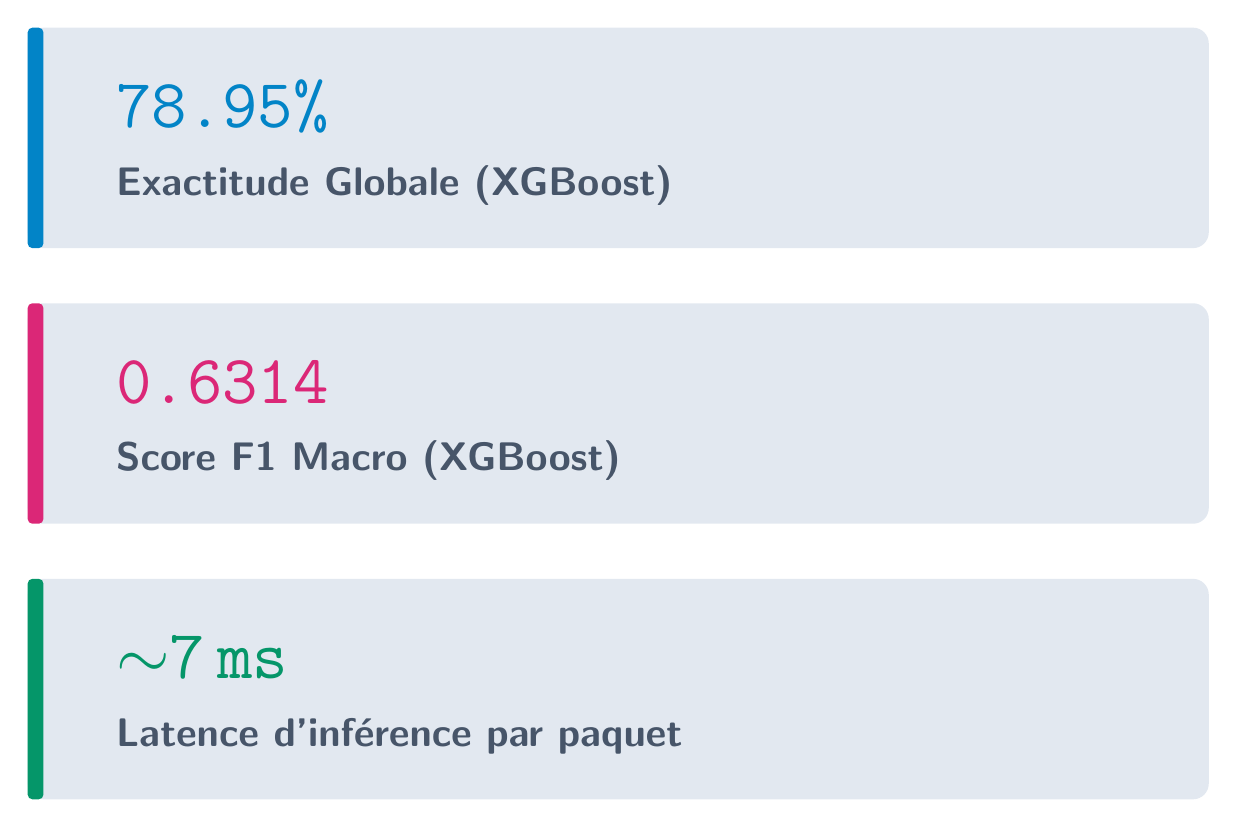
\begin{tikzpicture}[x=1mm,y=1mm]
  \foreach \y/\col/\val/\lab in {
    72/CyanAccent/{78.95\%}/{Exactitude Globale (XGBoost)},
    37/Magenta/{0.6314}/{Score F1 Macro (XGBoost)},
    2/NormalColor/{$\sim$7\,ms}/{Latence d'inf\'erence par paquet}}{
    \fill[PanelBgTitle, rounded corners=2mm] (0,\y) rectangle (150,\y+28);
    \fill[\col, rounded corners=0.6mm] (0,\y) rectangle (2,\y+28); % Barre accentuée
    \node[anchor=west, font=\metricfont, text=\col] at (10,\y+18) {\val};
    \node[anchor=west, font=\labelfont, text=TextMuted] at (10,\y+8) {\lab};
  }
\end{tikzpicture}
\end{center}
\vspace{2mm}
\end{tcolorbox}

\end{minipage}%
\hspace{\gapW}%
%% -------------------------------------------------------------
%%  COLUMN 3
%% -------------------------------------------------------------
\begin{minipage}[t]{\colW}

\begin{tcolorbox}[pc, title={\faTrophy\; R\'esultats D\'etaill\'es}]
\bodyfont\color{TextMain}
Les r\'esultats finaux du mod\`ele \textbf{XGBoost} sur l'ensemble de test NSL-KDD (22\,544 connexions).

\vspace{5mm}
{\labelfont\color{CyanAccent}Rapport de Classification~:}
\vspace{2mm}

{\smallfont
\setlength{\tabcolsep}{2.5mm}
\renewcommand{\arraystretch}{1.5}
\begin{tabular}{@{}lcccc@{}}
\rowcolor{TableHead}
  \textcolor{TextMain}{\textbf{Classe}} &
  \textcolor{TextMain}{\textbf{Pr\'ec.}} &
  \textcolor{TextMain}{\textbf{Rappel}} &
  \textcolor{TextMain}{\textbf{F1}} &
  \textcolor{TextMain}{\textbf{Support}} \\
\textcolor{NormalColor}{\textbf{Normal}} & 97.2\% & 98.1\% & 97.6\% & 9\,711 \\
\rowcolor{RowAlt}
\textcolor{DosColor}{\textbf{DoS}}       & 96.6\% & 98.0\% & 97.3\% & 7\,460 \\
\textcolor{ProbeColor}{\textbf{Probe}}   & 89.4\% & 84.2\% & 86.7\% & 2\,421 \\
\rowcolor{RowAlt}
\textcolor{R2LColor}{\textbf{R2L}}       & 97.1\% & \textcolor{DosColor}{\textbf{21.5\%}} & 35.0\%  & 2\,885 \\
\textcolor{U2RColor}{\textbf{U2R}}       & 71.9\% & \textcolor{DosColor}{\textbf{34.4\%}} & 46.0\%  &    67 \\
\end{tabular}
}

\vspace{5mm}
\begin{tcolorbox}[alert]
\smallfont\color{TextMain}
\textcolor{DosColor}{\faExclamationTriangle}\; \textbf{Point critique~:} le mod\`ele excelle sur \textbf{DoS} et \textbf{Probe}, mais le rappel R2L chute \`a \textbf{21.5\%} malgr\'e 97\% de pr\'ecision~--~la raret\'e extr\^eme (995 ex.) limite la g\'en\'eralisation malgr\'e SMOTE.
\end{tcolorbox}
\end{tcolorbox}

\vspace{5mm}

\begin{tcolorbox}[pc, title={\faDesktop\; Dashboard Temps R\'eel}]
\bodyfont\color{TextMain}
Nous avons d\'evelopp\'e une interface web moderne et r\'eactive pour simuler et surveiller le trafic r\'eseau en temps r\'eel.

\vspace{4mm}

\begin{center}
\begin{tikzpicture}[x=1mm,y=1mm]
  \draw[PanelBorder, line width=1.5pt, rounded corners=3mm] (0,0) rectangle (160,80);
  \node[anchor=center, inner sep=0pt] at (80,40) {\includegraphics[width=158mm,height=78mm,keepaspectratio]{dashboard.png}};
\end{tikzpicture}
\end{center}

\vspace{4mm}
{\labelfont\color{CyanAccent}Fonctionnalit\'es du Dashboard~:}
\begin{itemize}[leftmargin=6mm, itemsep=1.5mm, topsep=2mm]
  \citem{Backend robuste en \textbf{FastAPI}.}
  \citem{Pr\'ediction de flux asynchrones.}
  \citem{Visualisation des taux d'attaques en direct.}
  \citem{Solution enti\`erement conteneuris\'ee via \textbf{Docker}.}
\end{itemize}
\end{tcolorbox}

\vspace{5mm}

\begin{tcolorbox}[pc, title={\faLightbulb\; Conclusion \& Perspectives}]
\bodyfont\color{TextMain}
Ce projet d\'emontre l'efficacit\'e de \textbf{XGBoost} pour d\'etecter les intrusions r\'eseau classiques. L'int\'egration de SMOTE a permis d'att\'enuer le d\'es\'equilibre, mais les attaques sophistiqu\'ees (U2R) n\'ecessitent des approches diff\'erentes.

\vspace{4mm}
{\labelfont\color{CyanAccent}Perspectives d'\'evolution~:}
\begin{itemize}[leftmargin=6mm, itemsep=1.5mm, topsep=2mm]
  \citem{Utilisation de mod\`eles s\'equentiels (\textbf{LSTM}) pour capturer l'historique des paquets.}
  \citem{Mise \`a l'\'echelle sur le dataset \textbf{CICIDS2017}.}
  \citem{D\'eploiement sur mat\'eriel Edge (Edge AI).}
\end{itemize}
\end{tcolorbox}

\end{minipage}

\vspace{3mm}

%% =============================================================
%%  GRAPHS SECTION
%% =============================================================
\noindent
\begin{minipage}{570mm}
\begin{tcolorbox}[pc, title={\faChartArea\; Analyses Visuelles \& Performances du Mod\`ele}]
\vspace{1mm}
\begin{center}
\begin{tikzpicture}[x=1mm,y=1mm]
  \draw[PanelBorder, line width=1.5pt, rounded corners=3mm] (0,0) rectangle (260,104);
  \node[anchor=center, inner sep=0pt] at (130,59) {
\includegraphics[width=254mm,height=99mm,keepaspectratio]{confusion_matrices.png}};

  \begin{scope}[shift={(280,0)}]
    \draw[PanelBorder, line width=1.5pt, rounded corners=3mm] (0,0) rectangle (260,104);
    \node[anchor=center, inner sep=0pt] at (130,59) {
\includegraphics[width=254mm,height=99mm,keepaspectratio]{feature_importance.png}};
  \end{scope}
\end{tikzpicture}
\end{center}
\vspace{1mm}
\end{tcolorbox}
\end{minipage}

\vspace{3mm}

%% =============================================================
%%  TECHNOLOGIES SECTION
%% =============================================================
\noindent
\begin{minipage}{570mm}
\begin{tcolorbox}[pc, title={\faCode\; Technologies Utilis\'ees}]
\vspace{3mm}
\begin{center}
\begin{tikzpicture}[x=1mm,y=1mm]
  \tikzset{
    techbadge/.style={
      draw=CyanAccent, fill=RowAlt, line width=1.5pt, rounded corners=3mm,
      minimum width=90mm, minimum height=22mm, align=center,
      font=\fontsize{18}{22}\selectfont\bfseries, text=TextMain
    }
  }
  
  %% Les badges sont espacés uniformément sur une largeur totale de ~570mm
  \node[techbadge] at (57,0)  {\textcolor{CyanAccent}{\faPython}\; Python 3};
  \node[techbadge] at (171,0) {\textcolor{CyanAccent}{\faCogs}\; Scikit-Learn};
  \node[techbadge] at (285,0) {\textcolor{CyanAccent}{\faBolt}\; XGBoost};
  \node[techbadge] at (399,0) {\textcolor{CyanAccent}{\faServer}\; FastAPI};
  \node[techbadge] at (513,0) {\textcolor{CyanAccent}{\faDocker}\; Docker};

\end{tikzpicture}
\end{center}
\vspace{2mm}
\end{tcolorbox}
\end{minipage}

%% Permet de distribuer l'espace vide dynamiquement et de coller le footer tout en bas
\vfill 

%% =============================================================
%%  CONTACT FOOTER
%% =============================================================
\noindent
\begin{tikzpicture}[x=1mm,y=1mm]
  \fill[PanelBg, rounded corners=4mm] (0,0) rectangle (570,32);
  \draw[PanelBorder, rounded corners=4mm, line width=1.5pt] (0,0) rectangle (570,32);
  \draw[CyanAccent, line width=2pt] (3,31) -- (567,31);

  \node[text=TextMain, font=\fontsize{16}{20}\selectfont\bfseries, anchor=center] at (127.5, 21) {Sifeddine Legnioui};
  \node[text=TextMuted, font=\fontsize{12.5}{16}\selectfont, anchor=center] at (127.5, 9) {\textcolor{CyanAccent}{\faEnvelope}\; Sifeddine.legnioui-etu@etu.univh2c.ma \quad \textcolor{CyanAccent}{\faLinkedin}\; /in/seif-eddine-legnioui-5990b2297};

  \draw[PanelBorder, line width=1.2pt, dashed] (255, 4) -- (255, 28);

  \node[text=TextMain, font=\fontsize{16}{20}\selectfont\bfseries, anchor=center] at (382.5, 21) {Youssef Sarraf};
  \node[text=TextMuted, font=\fontsize{12.5}{16}\selectfont, anchor=center] at (382.5, 9) {\textcolor{CyanAccent}{\faEnvelope}\; youssef.sarraf-etu@etu.univh2c.ma \quad \textcolor{CyanAccent}{\faLinkedin}\; /in/youssef-sarraf};

  \draw[PanelBorder, line width=1.2pt, dashed] (510, 4) -- (510, 28);

  \fill[white, rounded corners=1.5mm] (523, 2.5) rectangle (552, 29.5);
  \node[anchor=center] at (537.5, 16) {\includegraphics[width=24mm,height=24mm,keepaspectratio]{qr_github.png}};
\end{tikzpicture} 

\end{document}